\section{HTLC limit in the Lightning Network}
\label{sec:attack}

In this section, we describe a limitation in the LN design 
stemming from the way it manages concurrent payments. 
A payment channel, even with sufficient capacity, can hold only 
a certain number of concurrent payments (governed by HTLCs), leading to capacity under-utilization. 
%While concurrent payments are theoretically 
%limited by the capacity (i.e., number of satohsis) in the channel, in practice 
%they are limited to a lower number that leads to capacity under-utilization. 
We study the effect of this limitation.
First, we evaluate how the number of concurrent payments in LN 
is majoritarily bounded by the number of concurrent HTLCs allowed at each channel. 
Second, we show how a malicious node can abuse this 
limitation to isolate parts of the network, 
which ultimately results in a network-wide DoS attack.
We provide estimates for the cost of such an attack, showing that it is within range for a moderately resourceful attacker. 
We finally discuss potential countermeasures.

\subsection{Background} \label{max-htlc-background}

Among other transaction validity rules, a Bitcoin transaction must be smaller than 100~KB (transaction size limit\cite{StandardTxBitcoinSE, BitcoinCoreMaxTxWeight}).\footnote{Bitcoin~Core, the reference Bitcoin implementation, defines a \textit{standard} transaction. Transaction size limit is a part of this definition. While non-standard transactions may be valid according to the consensus rules, Bitcoin~Core nodes do not propagate them. As Bitcoin~Core nodes constitute $97\%$ of the network~\cite{CoinDance}, non-standard transactions are highly unlikely to get confirmed.}
An LN channel can not contain more than 966~unsettled HTLCs, as prescribed in~\cite{BOLT2Rationale}.
This limit ensures that both counterparties can close the channel using one valid Bitcoin transaction.\footnote{The specification also points out that this limit ensures that the related messages conform to the limitation of the LN protocol, which limits the size of a message to $65535$~bytes.}
Hereby we refer to the limitation described above as the \textit{HTLC limit}.

Despite the perceived focus on micropayments, LN does not fully support transactions of very small value.
Every HTLC makes the potential closing transaction larger, and the on-chain fees higher.
Redeeming very small outputs on-chain can be more expensive than their value.
Therefore BOLT specifications prescribe that nodes negotiate the \textit{dust limit} before opening a channel, and for payments below this limit, no HTLCs are created (see \textit{trimmed HTLCs}~\cite{BOLT3Trimmed}).
%They are added to on-chain fees in case the channel closes at the current state.
Out of the three most popular LN implementations, c-lightning and Eclair use the default dust limit of $546$~satoshis.
LND estimates the dust limit dynamically.
We thus hereby assume $546$~satoshis as the dust limit.


%This effectively restricts the amount of information that a transaction can contain.

\subsection{Estimating the HTLC limit effect on LN scalability}	\label{estimating-concurrent channel updates}

In this section, we estimate the effect of the HTLC limit on the number of concurrent channel updates.
%In particular, we calculate an upper bound of the number of concurrent channel updates with and without the HTLC limit.
%We derive thereby the effect of the HTLC limit on the LN performance.

%\paragraph{Concurrent channel updates}
%Consider a channel with a capacity $c$.
%Given a transaction amount $a$, this channel can perform $c / a$ updates concurrently.
%However, given the HTLC limit, the number of concurrent updates is at most 966 (483 in each direction).

%We estimate the effect of the HTLC limit on the network performance by comparing the network-wide limit on the number of concurrent updates without the limit, i.e.,~based on the capacity alone ($u_{cap}$), and with the HTLC limit ($u_{HTLC}$).

Let $D$ be the dust limit.
We only consider amounts higher than $D$.
Let $C$ be the total network capacity (i.e., the sum of the individual capacities of all channels).
Let $a_\textit{avg}$ be the average transaction amount. 
Then, we say that the limit on concurrent updates based solely on capacity is defined as   
$u_\textit{cap} := C / a_\textit{avg}$.
In contrast, the limit on concurrent updates 
considering the HTLC limit is $u_\textit{HTLC} = N * 966$.
where $N$ is the number of channels. We remark here that $u_\textit{HTLC}$ does not depend on transaction amounts.

Given those two values, we define the 
\textit{effective update rate} $ur_\textit{eff}$ as the ratio between the actual limit on concurrent 
transactions when considering the HTLC limit and the theoretical 
limit based solely on capacity:

\[ur_\textit{eff} = \frac{min(u_\textit{cap}, u_\textit{HTLC})}{u_\textit{cap}}\]

Note that the effective update rate $ur_\textit{eff}$ depends on 
the average transaction amount, as shown in Figure~\ref{fig:effective-channel-updates}.
%For very low amounts, the effective number of concurrent updates is at the theoretical maximum.
Starting from $D$, there is a gap between the effective number of concurrent updates and what could be theoretically possible in the absence of the HTLC limit. 
%For instance, $ur_\textit{eff} = 37.43\%$ for $1000$~satoshis ($0.08$~USD) and $3.81\%$ for $100$~satoshis ($0.008$~USD).
We observe that $2677$ satoshis ($0.24$~USD) is the \textit{borderline amount}: for higher average transaction amounts, 
the limiting factor for the number of concurrent channel updates is channel capacity.
For amounts between $D$ and $2677$ satoshis, the limiting factor is the HTLC limit.
%For transactions with higher value than $2677$~satoshis LN is limited by capacity, 
%and for transactions of lower value the restriction on the number of in-flight HTLCs is the limiting factor.

\begin{figure}
	\centering
	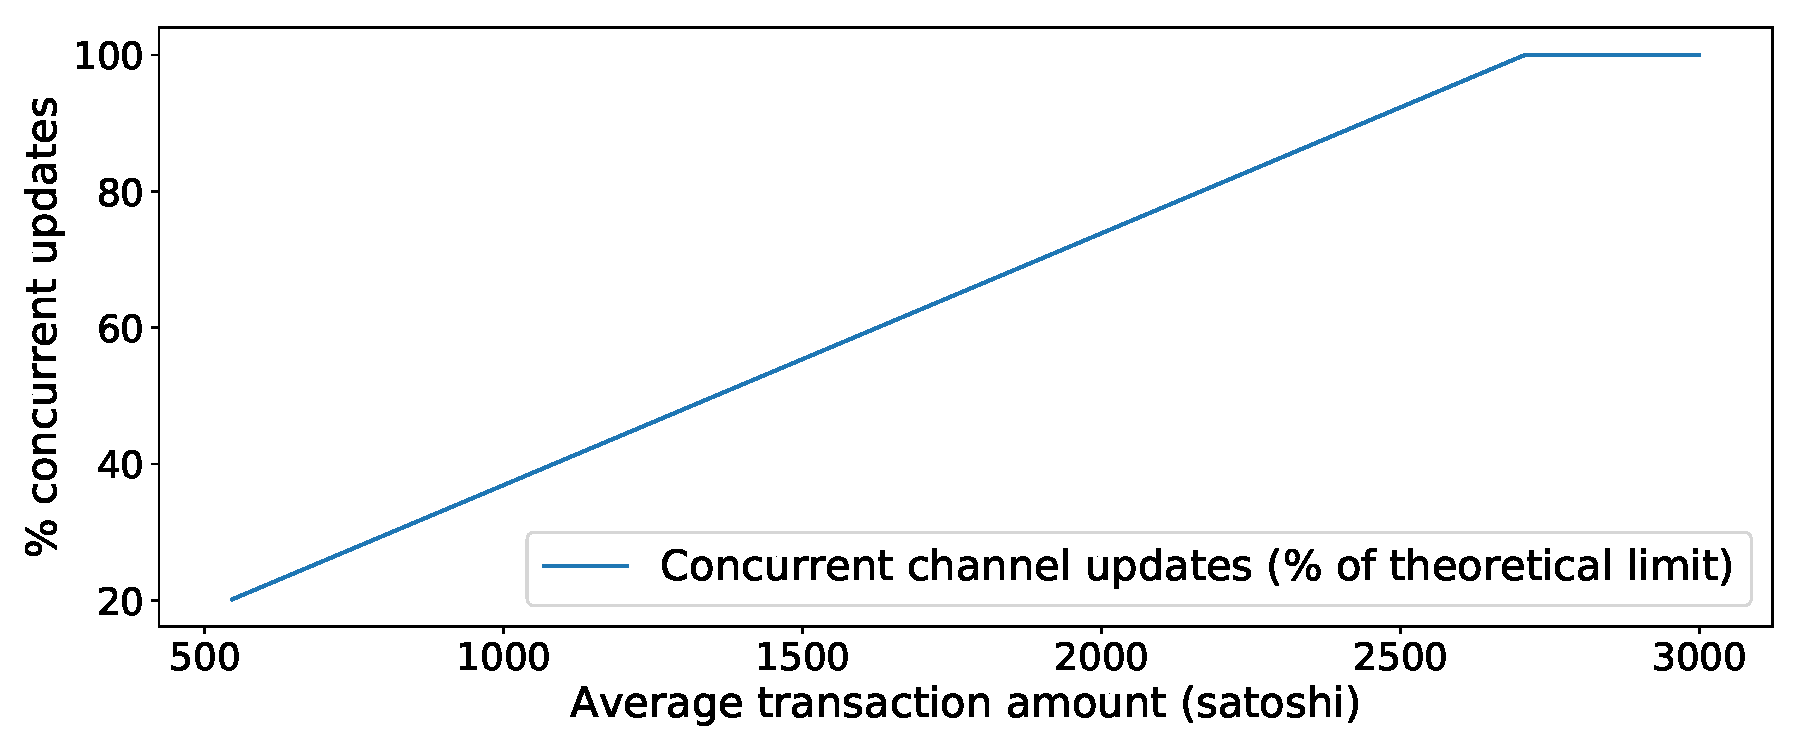
\includegraphics[width=\columnwidth]{effective-channel-updates}
	\caption{Ratio between the current limit on concurrent channel updates and the theoretically possible 
	capacity-based limit.\label{fig:effective-channel-updates}}
\end{figure}

\subsubsection*{Affected channels}
The $ur_\textit{eff}$ is an aggregated measurement that does not shed 
light on how the issue affects individual channels.  
Given that, we now study how many channels are affected by the HTLC limit.
The number of affected channels depends on the average transaction amount $a_\textit{avg}$. 
For high values of $a_\textit{avg}$, it is more likely that 
the effective update rate of a channel is limited by its capacity, 
whereas the HTLC limit would determine the update rate cap for small values of $a_\textit{avg}$.
We quantify this as follows.
Given a fixed average transaction amount $a_\textit{avg}$, 
we consider a channel \textit{affected} by the HTLC limit if $u_{\textit{HTLC},a_\textit{avg}} < u_{\textit{cap},a_\textit{avg}}$, i.e, $u_{\textit{eff},a_\textit{avg}} < 100\%$ (\cref{fig:affected-channels}).
%Note that contrary to network-wide calculations in the previous paragraph, here we consider the capacity of each channel individually.
%As in~\cref{fig:effective-channel-updates}, amounts lower than the dust limit have no effect on the network's throughput.
%$88.0\%$ of channels are affected with $a_\textit{avg}=100$, and $44.72\%$ are affected for $a_\textit{avg}=1000$.
%Drops on the graph correspond to popular channel capacities (?).

\begin{figure}
	\centering
	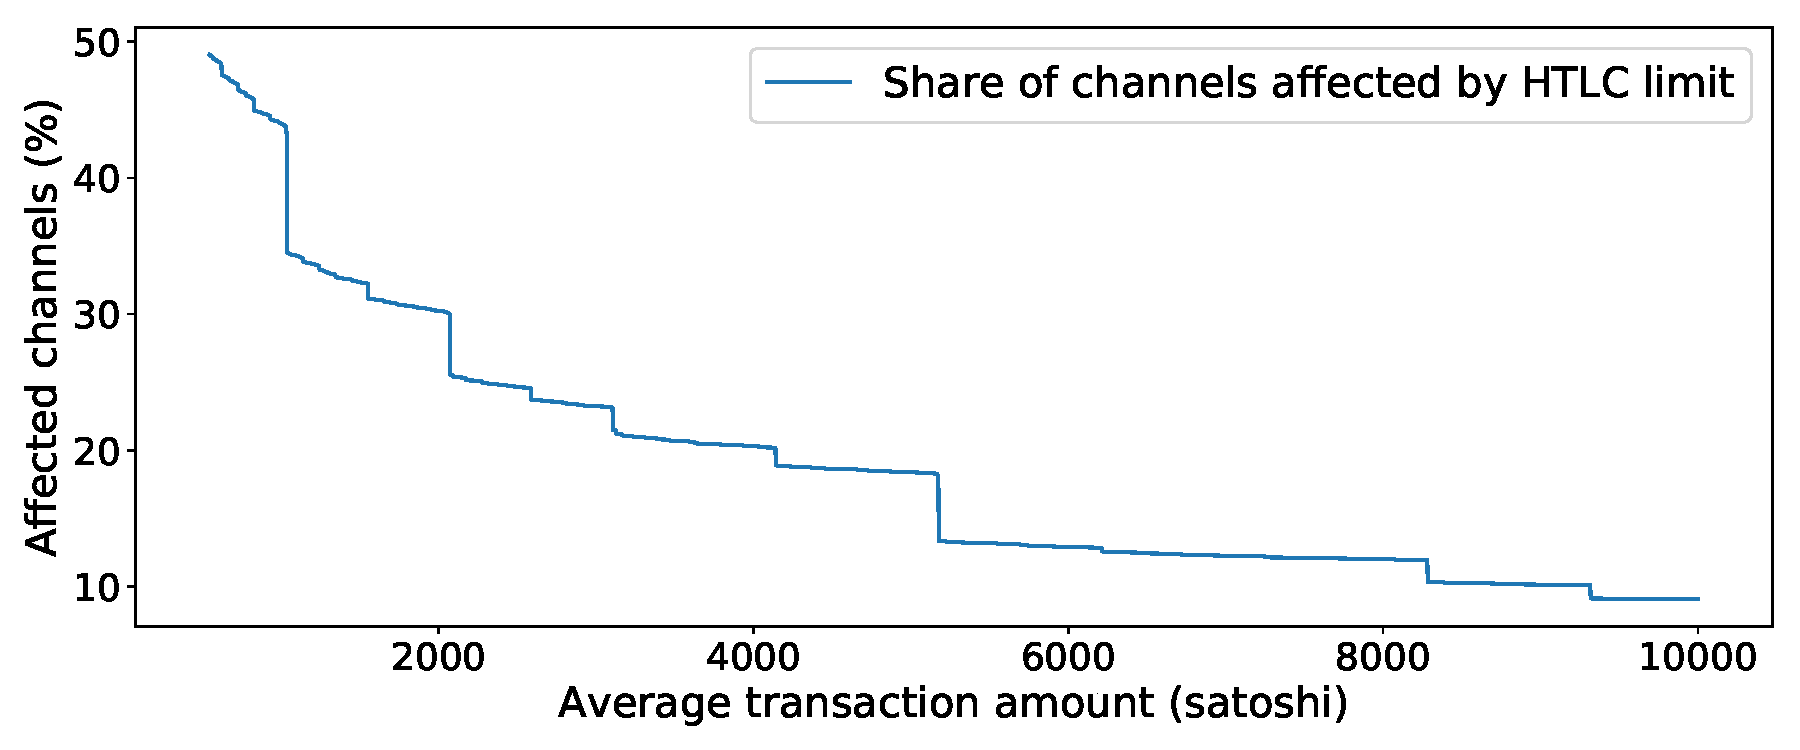
\includegraphics[width=\columnwidth]{affected-channels}
	\caption{Share of channels affected by the HTLC limit for different transaction amounts. \label{fig:affected-channels}}
\end{figure}



\subsubsection*{The effect of the HTLC limit over time}

%We use the set of historic snapshots (LNHist) to study how LN throughput changed over time.
%The dynamics regarding TPS limits shoes that the network throughput continues to grow with the increasing capacity and the number of channels.
%However, not enough channels (hence, HTLC slots) are being added to LN to accommodate the growing capacity.
%Therefore, LN performance is being held back by the HTLC limit for even smaller amount, as seen on Figure~\ref{fig:historic-tps}.
%\begin{figure}
%	\centering
%	\includegraphics[width=\columnwidth]{figures/historic-tps}
%	\caption{Historic TPS limits.\label{fig:historic-tps}}
%\end{figure}

We study the effect of the HTLC limit on the LN using our historical snapshots \emph{LNHist}.
For each monthly snapshot and four assumed average transaction amounts, we calculate the share of channels affected by the HTLC limit (\cref{fig:historic-htlc-limited-share}).
As expected, the HTLC limit becomes a more pressing issue 
with smaller transaction amounts, if they are higher than the dust limit.
We also observe that the share of affected channels has been increasing in the early months of LN and has remained stable since mid-2019.

We finally study how the \textit{borderline amount} has changed over time. 
%-- the average transaction amount for which the restriction on concurrent payments imposed by channel capacities is equal to the HTLC limit -- 
As~\cref{fig:historic-borderline-amount} shows, the HTLC limit finds 
its inflexion point in transaction amount at approximately $2500$~satoshis, with the borderline amount stabilizing in mid-2019, after the initial growth.

\begin{figure}[tb]
	\centering
	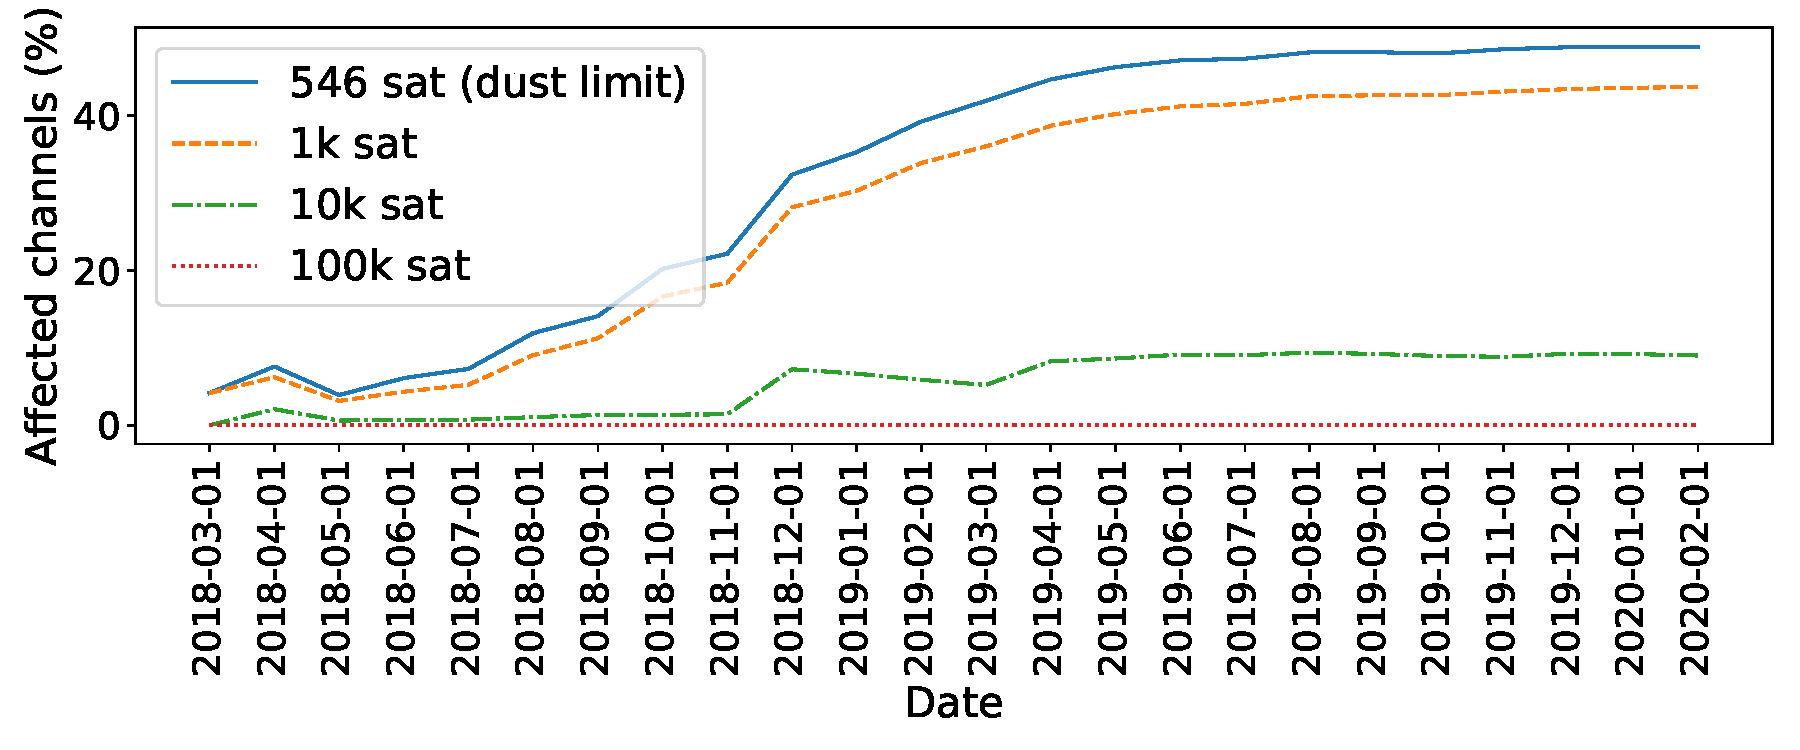
\includegraphics[width=\columnwidth]{historic-htlc-limited-share}
	\caption{Historic share of HTLC-limited channels.\label{fig:historic-htlc-limited-share}}
\end{figure}

\begin{figure}[tb]
	\centering
	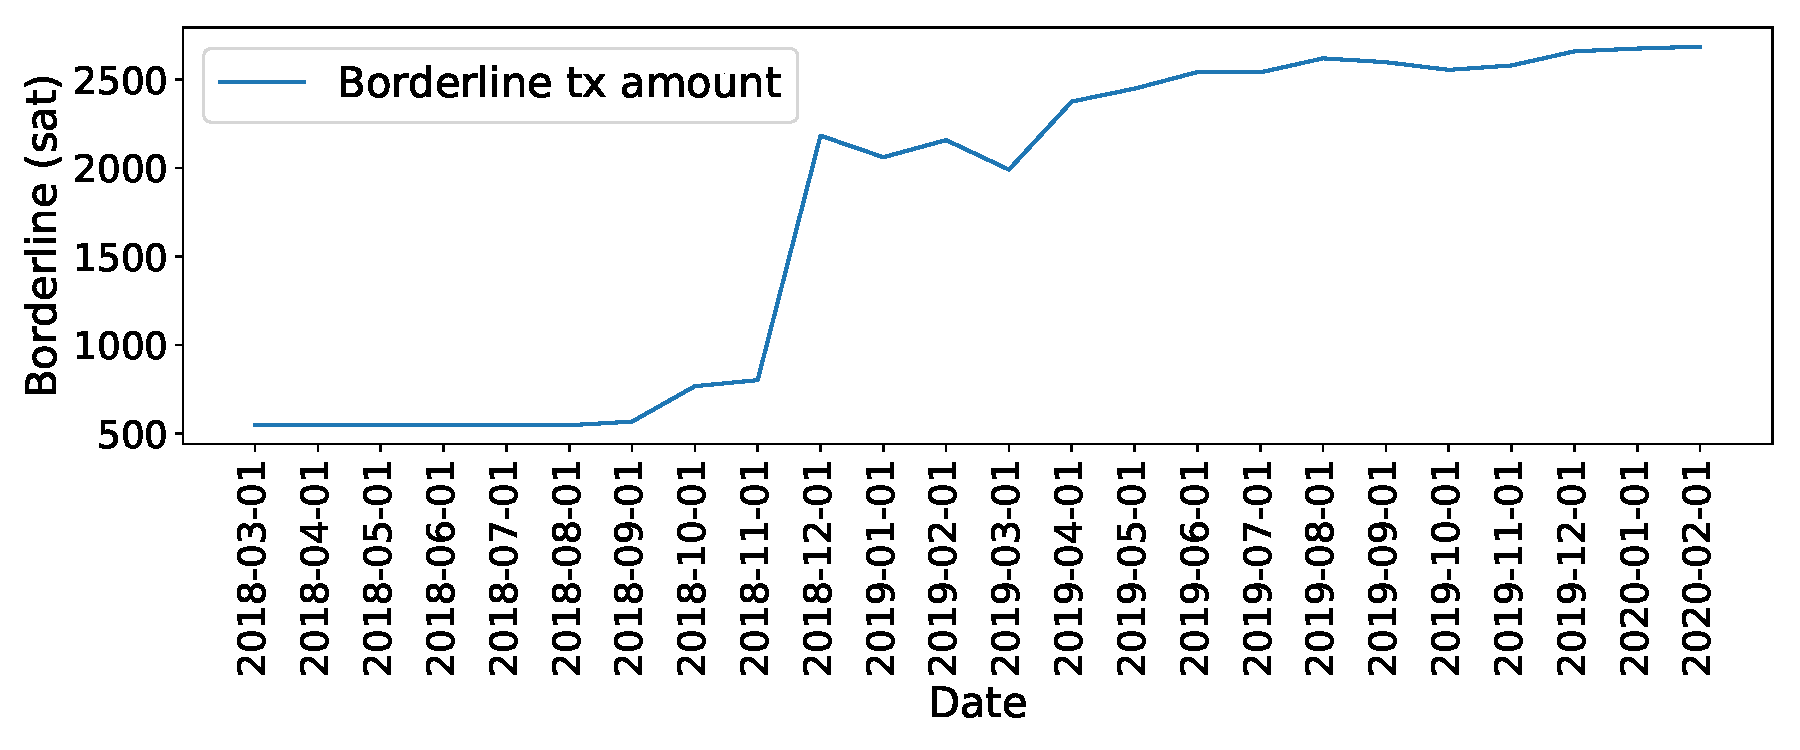
\includegraphics[width=\columnwidth]{historic-borderline-amount}
	\caption{Historic borderline amounts.\label{fig:historic-borderline-amount}}
\end{figure}



\subsection{Depleting the Lightning Network}

The HTLC limit opens up the possibility of a network-wide DoS attack.
An adversary connects to both endpoints of the target channel and forwards multiple small payments to itself, 
but does not finalize them.
After $966$ HTLCs are added, the channel loses its ability to forward payments, until some HTLCs expire. 
The attacker can thereby deplete a channel, making it unusable.

The cost for this attack depends on the minimum transaction amount.
% allowed by the channel and the dust limit.
%These values are set at the time of channel creation and can be later modified by the counterparties.
%From our dataset \textit{LN20}, the average minimum transaction amount is $1.273$~satoshis.
%Only $61$ out of more than $62$~thousand channel endpoints declare a minimum transaction amount higher than $1$~satoshi (the default setting in popular LN implementations).
We assume it equal to the dust limit of $546$~satoshis (the default value in 2 out of 3 major implementations).

We calculate the total capital requirements for an attacker to block the complete LN.
To block all $31084$~channels, the attacker would send, in the worst case, $966$ transactions of $546$ satoshi to each channel.
This brings the total capital requirements to approximately $163.9482$~BTC ($1.64M$~USD).

Each HTLC defines a timeout, after which the funds are returned to the sender, if the receiver provides no preimage.
From our dataset, we see that HTLC timeouts are long: $75.44$ blocks on average.
At a block creation rate of $10$~minutes per block, this implies that an average HTLC can block the capacity for around $12$~hours.
This implies that the attacker can render channels useless for around $12$~hours using the same HTLC parameters as regular LN users.
% Re-calculated in SQLite, 2020-02-25 data
%\todo[inline]{Pedro: These 12 hours number needs to be explained. Sergei: explained, is it OK?}


While this rough upper bound estimate suggests a rather high attack cost, the following optimizations make it more affordable.


\subsubsection*{Targeting highest-capacity channels}
The attack impact can be maximized by targeting highest-capacity channels.
For example, it requires $0.05$~BTC to block 10~top channels with combined capacity of $17.91$~BTC (\cref{fig:block-top-channels}).

\begin{figure}[tb]
	\centering
	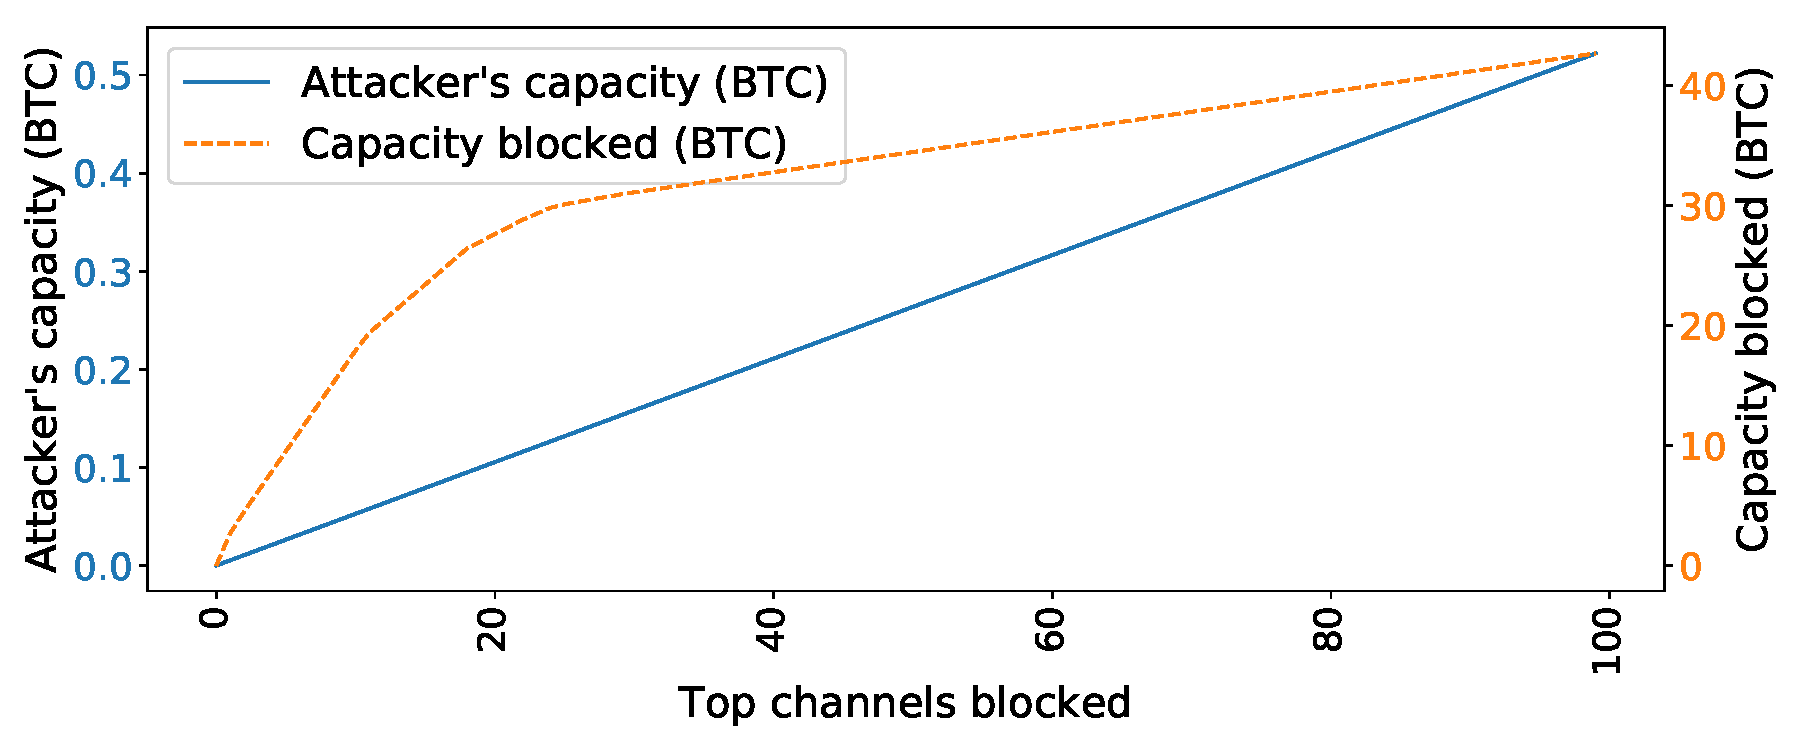
\includegraphics[width=\columnwidth]{block-top-channels}
	\caption{Effectiveness of targeting highest-capacity channels.\label{fig:block-top-channels}}
\end{figure}

\subsubsection*{Real HTLC limit}
Our calculations above are based on the maximum number of concurrent HTLC as defined by BOLT specifications ($483$).
LN implementations may choose lower default values for this parameter.
In particular, Eclair and c-lightning enforce a lower default HTLC limit ($30$).
%The third major implementation -- LND -- supports $483$~concurrent HTLCs per channel.
This means that in the real network the attacker needs to create fewer HTLCs to block channels between c-lightning and Eclair nodes as opposed to theoretical calculations and LND nodes (which by default support $483$ concurrent HTLCs per channel).
LND makes up $91\%$ of the nodes in the network, and Eclair is another $1\%$~\cite{Mizrahi2020}.
That brings real average HTLC limit to $442.23$ and lowers the attack cost by~$8.44\%$.
%\todo[inline]{Pedro: I don't understand this paragraph. Sergei: Now it's good?}

\subsubsection*{Multi-hop transactions}
The estimation above assumes single-hop transactions.
An attacker can leverage multi-hop transactions to multiply the effect of the committed capital,
connecting to both ends of a $20$-hop~\cite{Bolt4OnionRouting} payment path and performing a payment 
to itself that never gets completed. 
This is similar to capacity-based griefing attacks~\cite{HerreraJoancomarti2019}, 
but with much lower capital requirements.

\subsubsection*{Optimizing the attack based on communities}
The attacker may wish to prevent different parts of the network from transacting to each other.
To evaluate this possibility, we first divide the network into \textit{communities} using the Clauset-Newman-Moore greedy modularity maximization algorithm~\cite{Clauset2004}.
%LN graph can be divided into 25~communities.
Then we consider a scenario where the attacker tries to block the channels that connect communities 
rather than channels within communities.
For a chosen number $N$ of the largetst communities, we calculate how many channels the attacker has to block to split the network into at least $N+1$ parts: the $N$ largest communities and the rest of the network (\cref{fig:isolate-communities}).
We observe, e.g.,~that the attacker needs to block $4670$ channels 
($13\%$~of all channels) to isolate the largest community from the rest of the network, locking up $25$~BTC ($225k$~USD) -- or just around $2.8\%$~of the total LN capacity.
%\todo[inline]{Pedro: This number is a little discouraging. Shall we put it as a percentage of the total capital in the LN instead?}

\begin{figure}[tb]
	\centering
	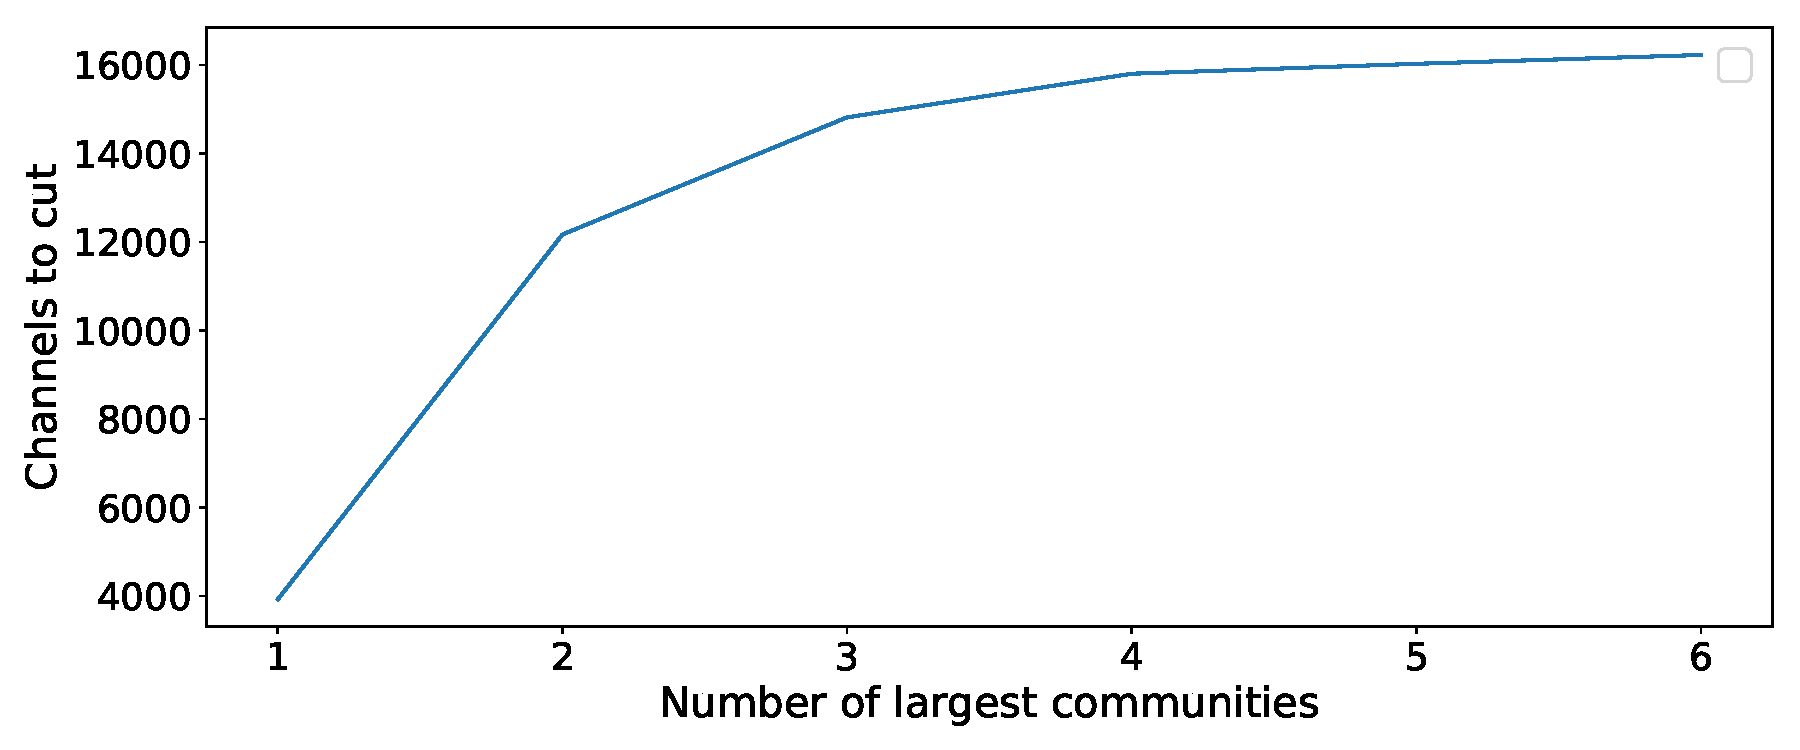
\includegraphics[width=\columnwidth]{isolate-communities}
	\caption{Number of channels to cut to isolate the largest communities.\label{fig:isolate-communities}}
\end{figure}



\subsection{Discussion}
Our simplistic model does not fully reflect all the details of transaction handling. 
In particular, we do not account for the fact that transactions take multiple hops (and multiple failed paths) before succeeding, nor do we reflect the unequal forwarding ability of a unit of capacity at a well-connected node, 
as opposed to a poorly connected one.
We also do not account for non-public channels, which may account for $28\%$~of all channels~\cite{BitMEXPrivateChannels}.
Yet, our approach allows us to calculate the effect of the HTLC limit,
as both estimations (capacity-based limit and HTLC limit) are calculated under the same assumptions.
Our estimation shows that the HTLC limit reduces the number of concurrent channel updates 
for payments under certain average transaction amount. 

The fact that the HTLC limit manifests itself at low transaction amounts negatively affects scalability.
Many potential LN applications involve transactions with tiny amounts.
The original Lightning paper~\cite{Poon2016} envisions use cases such as paying for online content and internet traffic.
Our calculations show that for payments of $1000$~satoshis ($0.009$~USD),
the network-wide rate of concurrent channel updates is $60\%$ lower 
than it could have been based solely on capacity limitations.

The low value for the default minimum transaction amount and the reduced number of in-flight transactions  
open a DoS attack vector with a moderate cost for the adversary.
Note that the capital in the attacker's channels will be recouped after the HTLCs time out.
Moreover, the unequal distribution of connectivity in the current LN paves the way for optimized attacks 
where the attacker focuses on high-capacity or inter-community channels to disrupt the 
seamless transfer of value across the network.


\subsection{Countermeasures}
One of the limiting factors for transaction throughput is the total available capacity.
This limitation is overcome by opening new channels, 
a countermeasure that will be naturally implemented with the growing LN adoption. 
The issue of the HTLC limit is more challenging as it comes from the limitations of the Bitcoin and Lightning protocols themselves.
Therefore, more fundamental changes are needed to reduce the information required to  
carry out the functionality encoded in HTLCs.
One countermeasure involves replacing HTLC with AMHL~\cite{Malavolta2019}. 
While HTLC requires including a digital signature, a hash value and a timelock, AMHL contract only requires the digital signature and the timelock while providing the same functionality. 

%Another potential countermeasure is the planned Taproot update to Bitcoin~\cite{TaprootBIP}.
%This update would allow to implement the HTLC functionality more compactly using Schnorr signatures.
%\todo[inline]{Pedro: We could add taproot here.Sergei: is this accurate?}

This countermeasure would reduce the number of bytes required per in-flight transaction 
and increase the number of payments handled concurrently.
While not removing the limitation on the number of concurrent transactions, 
this countermeasure raises this limit, reducing its negative effect on LN scalability.

